
%----------------------------------------------------------------%
%--------------------------INFORMATIONEN-------------------------%
%----------------------------------------------------------------%
%	Infos gibt es zu jedem Paket auf www.ctan.org
%	Werden bei den Paketen bestimmte Optionen gesetzt, so sind die Wichtigsten erklaert
%	solange sie nicht selbsterklärend sind

%----------------------------------------------------------------%
%--------------------------GRUNDEINSTELLUNGEN--------------------%
%----------------------------------------------------------------%
\documentclass[oneside, ngerman]{scrartcl}
%	'oneside'/'twoside': nicht zwischen linker und rechter Seite unterscheiden (alternativ twoside)
%	'twocolumn': wuerde 2 Spalten auf dem Blatt platzieren
%	'bibliography=totocnumbered': Normal nummeriertes Inhaltsverzeichnis (Kapitelnummer)
%	'listof=totocnumbered': Abbildungs- und Tabellenverzeichnis normal nummeriert (Kapitelnummer)
%	'ngerman' verwendet deutsch als Dokumentensprache (z.B. fuer Sirange)

\usepackage[ngerman]{babel}							%	Einstellen der Sprache
\usepackage[T1]{fontenc}							%	Wie wird Text ausgegeben, d.h. im PDF
\usepackage[utf8]{inputenc}							%	Welche Zeichen 'versteht' LaTeX bei der Eingabe?
\usepackage{lmodern}								%	Laedt Schriften, die geglaettet sind
											
\usepackage{blindtext}								%	Beispieltext, zum Testen geeignet
\usepackage{subfigure}
%----------------------------------------------------------------%
%--------------------------SEITENLAYOUT--------------------------%
%----------------------------------------------------------------%
\usepackage[left=3cm,right=3cm]{geometry}			%	Paket, welches vielfaeltige Einstellungen zum Seitenlayout liefert

%----------------------------------------------------------------%
%--------------------------ABSTÄNDE------------------------------%
%----------------------------------------------------------------%
\usepackage[onehalfspacing]{setspace}				%	Für Zeilenabstaende: 'singlespacing' (einfach), 'onehalfspacing' (1.5-fach), 'doublespacing' (2fach)

%\setlength{\parindent}{0cm}						%	Laengenangabe für die Einrueckung der ersten Zeile eines neuen Absatzes.
%\setlength{\parskip}{6pt plus 3pt minus 3pt}		%	Laengenangabe für den Abstand zwischen zwei Absaetzen.
%	Wenn diese beiden Befehle nicht kommentiert sind, wird ein Absatz nicht eingezogen sondern es gibt einen Abstand

%----------------------------------------------------------------%
%--------------------------MATHE---------------------------------%
%----------------------------------------------------------------%
\usepackage[]{mathtools}							%	Erweiterung von AMSMath, laedt automatisch AMSMath - für viele Mathe-Werkzeuge, 'fleqn' als Option ist für Mathe linksbuendig
\usepackage{amsfonts}								%	Für eine Vielzahl an mathematischen Symbolen

%----------------------------------------------------------------%
%--------------------------KOPF- UND FUSSZEILEN------------------%
%----------------------------------------------------------------%
\usepackage[automark,headsepline=.4pt]{scrlayer-scrpage}
\pagestyle{scrheadings}
\setkomafont{pageheadfoot}{\normalfont\bfseries}	%	Normale Schriftart und Fett für den Seitenkopf
\addtokomafont{pagenumber}{\normalfont\bfseries}	%	Normale Schriftart und Fett für die Seitenzahl
\clearscrheadfoot
\rohead{\thepage}									%	Rechter Seitenkopf mit Seitenzahl, ungerade Seiten
\lehead{\thepage}									%	Linker Seitenkopf mit Seitenzahl, gerade Seiten
\lohead{\headmark}									%	Linker Seitenkopf mit section, ungerade Seiten
\rehead{\headmark}									%	Linker Seitenkopf mit section, gerade Seiten
\lefoot[\pagemark]{\empty}							%	Leere Fußzeile, ungerade Seiten
\rofoot[\pagemark]{\empty}							%	Leere Fußzeile, gerade Seiten
\setlength{\headheight}{1.1\baselineskip}			%	Hoehe der Kopfzeile definieren
%	Definert man oben in der documentclass 'twoside', so wird zwischen geraden und ungeraden Seiten unterschieden

%----------------------------------------------------------------%
%--------------------------BILDER--------------------------------%
%----------------------------------------------------------------%
\usepackage{graphicx}									%	Um Bilder einbinden zu koennen
\usepackage[usenames,dvipsnames,svgnames]{xcolor}		%	Um Farben verwenden zu koennen
\usepackage{pdfpages}									%	pdfs importieren

%----------------------------------------------------------------%
%--------------------------POSITIONIERUNG------------------------%
%----------------------------------------------------------------%
\usepackage{float}

%----------------------------------------------------------------%
%--------------------------LISTEN--------------------------------%
%----------------------------------------------------------------%
\usepackage{enumitem}							%	Um Listen / Aufzaehlungen leichter zu modifizieren
%\setlist{noitemsep}							%	Verringert den Abstand in Aufzaehlungen

%----------------------------------------------------------------%
%--------TABELLEN-/BILDUNTERSCHRIFTEN und NUMMERIERUNG-----------%
%----------------------------------------------------------------%
\usepackage[format=hang, indention=0mm, labelsep=colon, justification=justified,  labelfont=bf]{caption}
\setlength\parindent{0pt}
%	'format=hang': Platz unter Abb. X bleibt frei, 'format=plain': auch unter Abb. X befindet sich Text
%	'idention': Einzug der zweiten Textzeile
%	'labelsep=colon': Trenner zwischen Nr. und Text ist Doppelpunkt und Leerzeichen
%	'justification=justified': Text wird als Block gesetzt
%	'labelfont=bf': 'Abbildung X.X' wird fett geschrieben

\numberwithin{equation}{section}				%	Nummerierung der Gleichungen, Tabellen und Bilder nach der Kapitelnummer
\numberwithin{figure}{section}
\numberwithin{table}{section}

%----------------------------------------------------------------%
%--------------------------LITERATURVERZEICHNIS------------------%
%----------------------------------------------------------------%
\usepackage[german]{babelbib}					%	Bereitstellung des deutschen Layouts fuer die Bibliography

%----------------------------------------------------------------%
%--------------------------SIUNITX-------------------------------%
%----------------------------------------------------------------%
\usepackage[]{siunitx}
\sisetup{locale = DE}							%	Automatische Einstellung der Ausgabe für bestimmte Regionen (UK, US, DE, FR, ZA)

%----------------------------------------------------------------%
%--------------------------URLs / REFs---------------------------%
%----------------------------------------------------------------%
\usepackage[hidelinks]{hyperref}				%	Erweiterte Referenzierung ('hidelinks' verhindert Linien um Links)
\usepackage{gensymb}
\usepackage{subfigure}
\usepackage{ textcomp }
\usepackage{dsfont}
\usepackage{siunitx}
\usepackage{comment}
\usepackage{tikz}
\usepackage{epstopdf}
\usepackage{graphicx}
\usetikzlibrary{arrows.meta}
%----------------------------------------------------------------%
%--------------------------EIGENE BEFEHLE------------------------%
%----------------------------------------------------------------%
\DeclareSIUnit\parsec{pc}
\DeclareSIUnit\lightyear{ly}

 \begin{document}
 %---------------------------------------------------------------------------------------------%
 %------------------------------------------TITELSEITE-----------------------------------------%
 %---------------------------------------------------------------------------------------------%
 \title{Radioteleskopie}
 \subtitle{Physikalisches Fortgeschrittenenpraktikum an der Universität Konstanz}
 \author{Autoren: Philipp Gebauer und Simon Keegan \\ \large{Tutor: Stefan Schupp}}
 \date{Versuch durchgeführt am 13.05.2020}
 \maketitle
 \vspace{2.5 cm}
 \begin{abstract}
     \noindent \textbf{Abstract:}\\
     Place for the abstract. TODO!!
     \vspace{1cm}
     
     \end{abstract}
 \thispagestyle{empty}
 \newpage
 
 %---------------------------------------------------------------------------------------------%
 %------------------------------------------INHALTSVERZEICHNIS---------------------------------%
 %---------------------------------------------------------------------------------------------%
 \tableofcontents
 \thispagestyle{empty}
 \newpage
 \setcounter{page}{1}    
 %---------------------------------------------------------------------------------------------%
 %------------------------------------------DOKUMENTENKÖRPER-----------------------------------%
 %-----------------------------------------------------------
 
 %----------------------------------%
\section{Einleitung}
\section{Aufbau und Durchführung des Versuchs}
\begin{figure}[H]
    \centering
    % GNUPLOT: LaTeX picture with Postscript
\begingroup
  % Encoding inside the plot.  In the header of your document, this encoding
  % should to defined, e.g., by using
  % \usepackage[cp1252,<other encodings>]{inputenc}
  \inputencoding{cp1252}%
  \makeatletter
  \providecommand\color[2][]{%
    \GenericError{(gnuplot) \space\space\space\@spaces}{%
      Package color not loaded in conjunction with
      terminal option `colourtext'%
    }{See the gnuplot documentation for explanation.%
    }{Either use 'blacktext' in gnuplot or load the package
      color.sty in LaTeX.}%
    \renewcommand\color[2][]{}%
  }%
  \providecommand\includegraphics[2][]{%
    \GenericError{(gnuplot) \space\space\space\@spaces}{%
      Package graphicx or graphics not loaded%
    }{See the gnuplot documentation for explanation.%
    }{The gnuplot epslatex terminal needs graphicx.sty or graphics.sty.}%
    \renewcommand\includegraphics[2][]{}%
  }%
  \providecommand\rotatebox[2]{#2}%
  \@ifundefined{ifGPcolor}{%
    \newif\ifGPcolor
    \GPcolorfalse
  }{}%
  \@ifundefined{ifGPblacktext}{%
    \newif\ifGPblacktext
    \GPblacktexttrue
  }{}%
  % define a \g@addto@macro without @ in the name:
  \let\gplgaddtomacro\g@addto@macro
  % define empty templates for all commands taking text:
  \gdef\gplbacktext{}%
  \gdef\gplfronttext{}%
  \makeatother
  \ifGPblacktext
    % no textcolor at all
    \def\colorrgb#1{}%
    \def\colorgray#1{}%
  \else
    % gray or color?
    \ifGPcolor
      \def\colorrgb#1{\color[rgb]{#1}}%
      \def\colorgray#1{\color[gray]{#1}}%
      \expandafter\def\csname LTw\endcsname{\color{white}}%
      \expandafter\def\csname LTb\endcsname{\color{black}}%
      \expandafter\def\csname LTa\endcsname{\color{black}}%
      \expandafter\def\csname LT0\endcsname{\color[rgb]{1,0,0}}%
      \expandafter\def\csname LT1\endcsname{\color[rgb]{0,1,0}}%
      \expandafter\def\csname LT2\endcsname{\color[rgb]{0,0,1}}%
      \expandafter\def\csname LT3\endcsname{\color[rgb]{1,0,1}}%
      \expandafter\def\csname LT4\endcsname{\color[rgb]{0,1,1}}%
      \expandafter\def\csname LT5\endcsname{\color[rgb]{1,1,0}}%
      \expandafter\def\csname LT6\endcsname{\color[rgb]{0,0,0}}%
      \expandafter\def\csname LT7\endcsname{\color[rgb]{1,0.3,0}}%
      \expandafter\def\csname LT8\endcsname{\color[rgb]{0.5,0.5,0.5}}%
    \else
      % gray
      \def\colorrgb#1{\color{black}}%
      \def\colorgray#1{\color[gray]{#1}}%
      \expandafter\def\csname LTw\endcsname{\color{white}}%
      \expandafter\def\csname LTb\endcsname{\color{black}}%
      \expandafter\def\csname LTa\endcsname{\color{black}}%
      \expandafter\def\csname LT0\endcsname{\color{black}}%
      \expandafter\def\csname LT1\endcsname{\color{black}}%
      \expandafter\def\csname LT2\endcsname{\color{black}}%
      \expandafter\def\csname LT3\endcsname{\color{black}}%
      \expandafter\def\csname LT4\endcsname{\color{black}}%
      \expandafter\def\csname LT5\endcsname{\color{black}}%
      \expandafter\def\csname LT6\endcsname{\color{black}}%
      \expandafter\def\csname LT7\endcsname{\color{black}}%
      \expandafter\def\csname LT8\endcsname{\color{black}}%
    \fi
  \fi
    \setlength{\unitlength}{0.0500bp}%
    \ifx\gptboxheight\undefined%
      \newlength{\gptboxheight}%
      \newlength{\gptboxwidth}%
      \newsavebox{\gptboxtext}%
    \fi%
    \setlength{\fboxrule}{0.5pt}%
    \setlength{\fboxsep}{1pt}%
\begin{picture}(7200.00,5040.00)%
    \gplgaddtomacro\gplbacktext{%
    }%
    \gplgaddtomacro\gplfronttext{%
      \csname LTb\endcsname%%
      \put(963,1308){\makebox(0,0){\strut{}$-10$}}%
      \put(1773,1160){\makebox(0,0){\strut{}$-5$}}%
      \put(2583,1011){\makebox(0,0){\strut{}$0$}}%
      \put(3392,863){\makebox(0,0){\strut{}$5$}}%
      \put(4201,714){\makebox(0,0){\strut{}$10$}}%
      \put(2270,651){\rotatebox{-11}{\makebox(0,0){\strut{}azimuth offset in $\degree$}}}%
      \put(4427,746){\makebox(0,0)[l]{\strut{}$-10$}}%
      \put(4895,1004){\makebox(0,0)[l]{\strut{}$-5$}}%
      \put(5362,1261){\makebox(0,0)[l]{\strut{}$0$}}%
      \put(5830,1518){\makebox(0,0)[l]{\strut{}$5$}}%
      \put(6297,1775){\makebox(0,0)[l]{\strut{}$10$}}%
      \put(5903,960){\rotatebox{29}{\makebox(0,0){\strut{}altitude offset in $\degree$}}}%
      \put(920,1482){\makebox(0,0)[r]{\strut{}$300$}}%
      \put(920,1972){\makebox(0,0)[r]{\strut{}$400$}}%
      \put(920,2462){\makebox(0,0)[r]{\strut{}$500$}}%
      \put(920,2951){\makebox(0,0)[r]{\strut{}$600$}}%
      \put(920,3441){\makebox(0,0)[r]{\strut{}$700$}}%
      \put(122,2462){\rotatebox{90}{\makebox(0,0){\strut{}temperature in $\si{}{K}$}}}%
    }%
    \gplbacktext
    \put(0,0){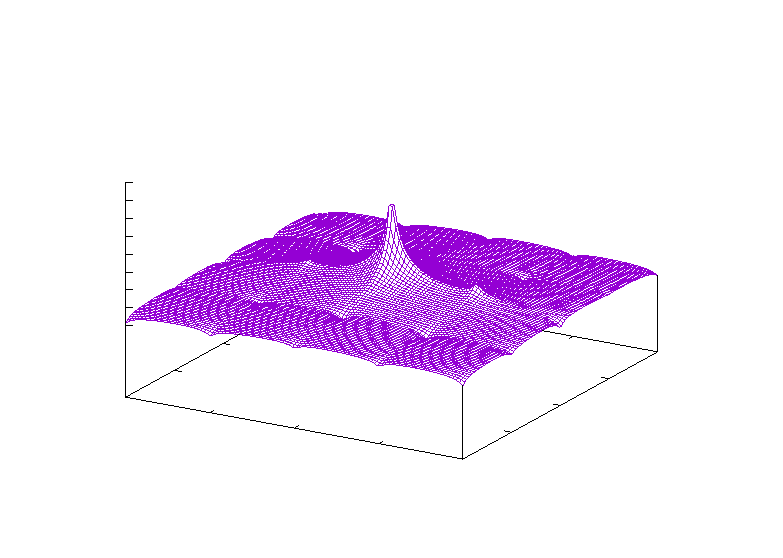
\includegraphics{plots/Sonnenabbild}}%
    \gplfronttext
  \end{picture}%
\endgroup

    \caption{todo}
    \label{fig:Sonnenabbild}
\end{figure}
Test2
 
     
\begin{figure}[H]
    \centering
    % GNUPLOT: LaTeX picture with Postscript
\begingroup
  % Encoding inside the plot.  In the header of your document, this encoding
  % should to defined, e.g., by using
  % \usepackage[cp1252,<other encodings>]{inputenc}
  \inputencoding{cp1252}%
  \makeatletter
  \providecommand\color[2][]{%
    \GenericError{(gnuplot) \space\space\space\@spaces}{%
      Package color not loaded in conjunction with
      terminal option `colourtext'%
    }{See the gnuplot documentation for explanation.%
    }{Either use 'blacktext' in gnuplot or load the package
      color.sty in LaTeX.}%
    \renewcommand\color[2][]{}%
  }%
  \providecommand\includegraphics[2][]{%
    \GenericError{(gnuplot) \space\space\space\@spaces}{%
      Package graphicx or graphics not loaded%
    }{See the gnuplot documentation for explanation.%
    }{The gnuplot epslatex terminal needs graphicx.sty or graphics.sty.}%
    \renewcommand\includegraphics[2][]{}%
  }%
  \providecommand\rotatebox[2]{#2}%
  \@ifundefined{ifGPcolor}{%
    \newif\ifGPcolor
    \GPcolorfalse
  }{}%
  \@ifundefined{ifGPblacktext}{%
    \newif\ifGPblacktext
    \GPblacktexttrue
  }{}%
  % define a \g@addto@macro without @ in the name:
  \let\gplgaddtomacro\g@addto@macro
  % define empty templates for all commands taking text:
  \gdef\gplbacktext{}%
  \gdef\gplfronttext{}%
  \makeatother
  \ifGPblacktext
    % no textcolor at all
    \def\colorrgb#1{}%
    \def\colorgray#1{}%
  \else
    % gray or color?
    \ifGPcolor
      \def\colorrgb#1{\color[rgb]{#1}}%
      \def\colorgray#1{\color[gray]{#1}}%
      \expandafter\def\csname LTw\endcsname{\color{white}}%
      \expandafter\def\csname LTb\endcsname{\color{black}}%
      \expandafter\def\csname LTa\endcsname{\color{black}}%
      \expandafter\def\csname LT0\endcsname{\color[rgb]{1,0,0}}%
      \expandafter\def\csname LT1\endcsname{\color[rgb]{0,1,0}}%
      \expandafter\def\csname LT2\endcsname{\color[rgb]{0,0,1}}%
      \expandafter\def\csname LT3\endcsname{\color[rgb]{1,0,1}}%
      \expandafter\def\csname LT4\endcsname{\color[rgb]{0,1,1}}%
      \expandafter\def\csname LT5\endcsname{\color[rgb]{1,1,0}}%
      \expandafter\def\csname LT6\endcsname{\color[rgb]{0,0,0}}%
      \expandafter\def\csname LT7\endcsname{\color[rgb]{1,0.3,0}}%
      \expandafter\def\csname LT8\endcsname{\color[rgb]{0.5,0.5,0.5}}%
    \else
      % gray
      \def\colorrgb#1{\color{black}}%
      \def\colorgray#1{\color[gray]{#1}}%
      \expandafter\def\csname LTw\endcsname{\color{white}}%
      \expandafter\def\csname LTb\endcsname{\color{black}}%
      \expandafter\def\csname LTa\endcsname{\color{black}}%
      \expandafter\def\csname LT0\endcsname{\color{black}}%
      \expandafter\def\csname LT1\endcsname{\color{black}}%
      \expandafter\def\csname LT2\endcsname{\color{black}}%
      \expandafter\def\csname LT3\endcsname{\color{black}}%
      \expandafter\def\csname LT4\endcsname{\color{black}}%
      \expandafter\def\csname LT5\endcsname{\color{black}}%
      \expandafter\def\csname LT6\endcsname{\color{black}}%
      \expandafter\def\csname LT7\endcsname{\color{black}}%
      \expandafter\def\csname LT8\endcsname{\color{black}}%
    \fi
  \fi
    \setlength{\unitlength}{0.0500bp}%
    \ifx\gptboxheight\undefined%
      \newlength{\gptboxheight}%
      \newlength{\gptboxwidth}%
      \newsavebox{\gptboxtext}%
    \fi%
    \setlength{\fboxrule}{0.5pt}%
    \setlength{\fboxsep}{1pt}%
\begin{picture}(7200.00,5040.00)%
    \gplgaddtomacro\gplbacktext{%
      \csname LTb\endcsname%%
      \put(814,704){\makebox(0,0)[r]{\strut{}$300$}}%
      \put(814,1218){\makebox(0,0)[r]{\strut{}$350$}}%
      \put(814,1733){\makebox(0,0)[r]{\strut{}$400$}}%
      \put(814,2247){\makebox(0,0)[r]{\strut{}$450$}}%
      \put(814,2762){\makebox(0,0)[r]{\strut{}$500$}}%
      \put(814,3276){\makebox(0,0)[r]{\strut{}$550$}}%
      \put(814,3790){\makebox(0,0)[r]{\strut{}$600$}}%
      \put(814,4305){\makebox(0,0)[r]{\strut{}$650$}}%
      \put(814,4819){\makebox(0,0)[r]{\strut{}$700$}}%
      \put(1434,484){\makebox(0,0){\strut{}$-15$}}%
      \put(2248,484){\makebox(0,0){\strut{}$-10$}}%
      \put(3061,484){\makebox(0,0){\strut{}$-5$}}%
      \put(3875,484){\makebox(0,0){\strut{}$0$}}%
      \put(4688,484){\makebox(0,0){\strut{}$5$}}%
      \put(5501,484){\makebox(0,0){\strut{}$10$}}%
      \put(6315,484){\makebox(0,0){\strut{}$15$}}%
      \put(4851,2813){\makebox(0,0)[l]{\strut{}FWHM $ = \SI{7.80 \pm 0.13}{\degree}$}}%
      \put(4851,3173){\makebox(0,0)[l]{\strut{}$\sigma =  \SI{3.313 \pm 0.055}{\degree}$}}%
    }%
    \gplgaddtomacro\gplfronttext{%
      \csname LTb\endcsname%%
      \put(308,2761){\rotatebox{-270}{\makebox(0,0){\strut{}Intensit\"at in willk\"urlichen Einheiten}}}%
      \put(3874,154){\makebox(0,0){\strut{}Azimutwinkelversatz relativ zur Sonne in $\si{}{\degree}$}}%
      \csname LTb\endcsname%%
      \put(5816,4646){\makebox(0,0)[r]{\strut{}Messwerte}}%
      \csname LTb\endcsname%%
      \put(5816,4426){\makebox(0,0)[r]{\strut{}\textsc{Gauss}-Fit}}%
    }%
    \gplbacktext
    \put(0,0){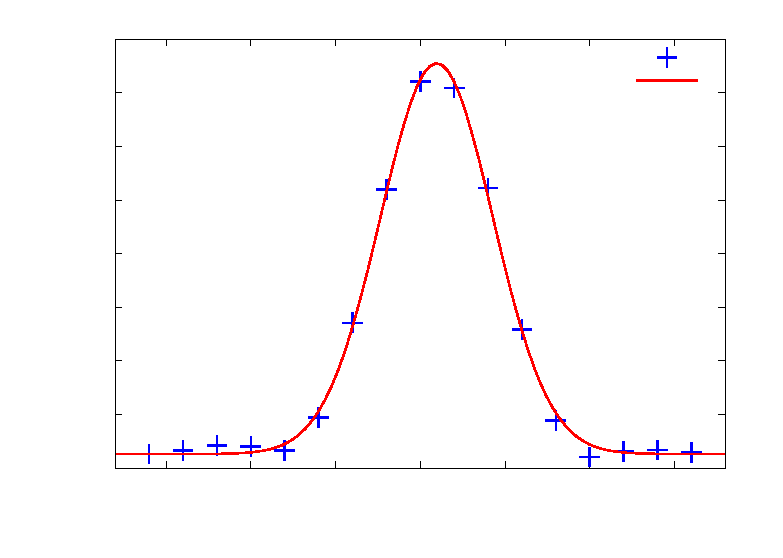
\includegraphics{plots/Sonnenkreuz_Az}}%
    \gplfronttext
  \end{picture}%
\endgroup

    \caption{todo}
    \label{fig:Sonnenkreuz_Az}
\end{figure}

     \newpage
     \bibliography{literatur}
 \bibliographystyle{babalpha}
 \listoffigures
 
 \end{document}
 